In parallelo sono state verificate le performance di CUTE valutando diverse situazioni.
In primo luogo, è stato valutato il tempo di esecuzione rispetto alle configurazioni già presentate nella \cref{subsec:comp:cluster}.
Successivamente sono stati eseguiti test per valutare le tempistiche al variare del numero di risorse fisiche impiegate, ovvero executor e core.
In tutti i test il tempo è sempre registrato in millisecondi.

Nel cronometrare la durata dell'algoritmo, non è considerata la fase di creazione delle tabelle di supporto.
Questo perché le tabelle in questione possono potenzialmente essere create separatamente da CUTE e poi utilizzate dall'algoritmo.
Inoltre a parità di parametri \(s\) e \(t\) una stessa tabella può essere utilizzata da più esecuzioni dell'algoritmo.

Partendo dalle valutazioni basate sull'alterazione dei parametri dell'algoritmo, la \cref{fig:chap-4:TimeSandT} mostrano il tempo di calcolo rispetto alle variazioni dei lati spazio-temporali della cella.
Al crescere di \(s\) (\cref{fig:chap-4:TimeS}), cala il tempo di esecuzione.
Intuitivamente ciò è collegato al numero di celle: celle più grandi e meno numerose corrispondono a meno transazioni da valutare durante la ricerca.
Per \(t\) (\cref{fig:chap-4:TimeT}) la situazione è diversa.
Il trend è inversamente proporzionale al numero di celle: al calare di queste, aumentano i tempi di esecuzione.
Nonostante quindi il numero di celle sia maggiore all'inizio con \(t=24h\), la minor lunghezza delle transazioni porta a generare un minor numero di gruppi da esplorare (come evidenziato anche negli itemset individuati) e causa quindi una diminuzione nei tempi di esecuzione.

\begin{figure}
  \centering
  \begin{subfigure}{.5\textwidth}
  \centering
   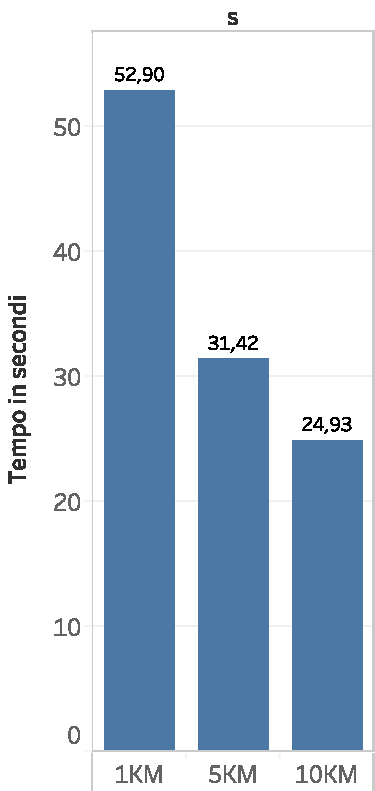
\includegraphics[scale=0.5]{res/fig/sec-4/performance/TimeS.pdf}
   \caption{\(s\) tra \(1,5,10\) KM}
  \label{fig:chap-4:TimeS}
\end{subfigure}%
\begin{subfigure}{.5\textwidth}
  \centering
   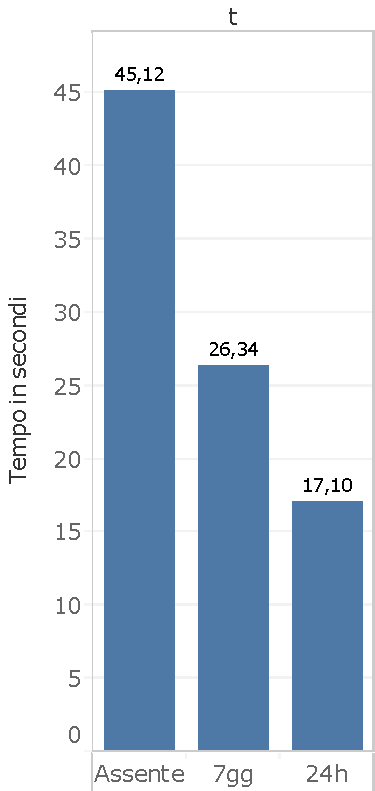
\includegraphics[scale=0.5]{res/fig/sec-4/performance/TimeT.pdf}
   \caption{\(t\) tra 24h, 7gg e assenza di tempo}
  \label{fig:chap-4:TimeT}
\end{subfigure}%
  \caption{Tempo di computazione alla variazione di \(s\) a sinistra, \(t\) a destra}%
  \label{fig:chap-4:TimeSandT}
\end{figure}

Variando \(minsize\) (\cref{fig:chap-4:TimeMinsize}) è possibile vedere un trend di diminuzione dei tempi di esecuzione al crescere del parametro.
Questo è coerente con quanto atteso: la ricerca di gruppi più numerosi comporta il pruning dei piccoli gruppi e risparmia tempo sul tempo di esecuzione globale.
Considerando invece \(minsup\) (\cref{fig:chap-4:TimeMinsupp}), vale lo stesso discorso.
Le ragioni sono analoghe a quanto detto per \(minsize\).


\begin{figure}
  \centering
   \begin{subfigure}{.5\textwidth}
  \centering
    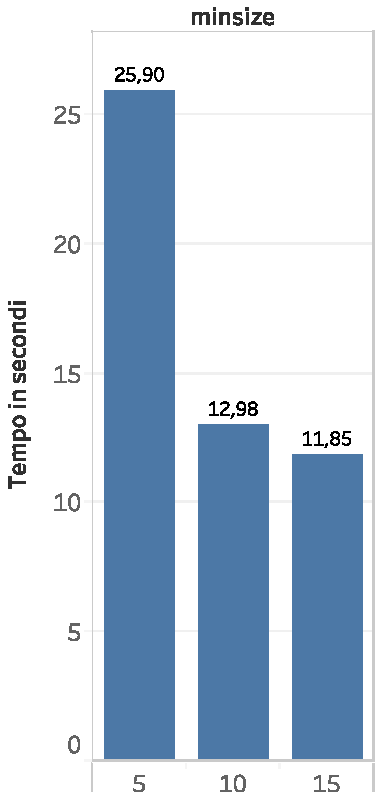
\includegraphics[scale=0.5]{res/fig/sec-4/performance/TimeMinsize.pdf}
   \caption{\(minsize\) tra \(5,10,15\)}
  \label{fig:chap-4:TimeMinsize}
\end{subfigure}%
\begin{subfigure}{.5\textwidth}
  \centering
   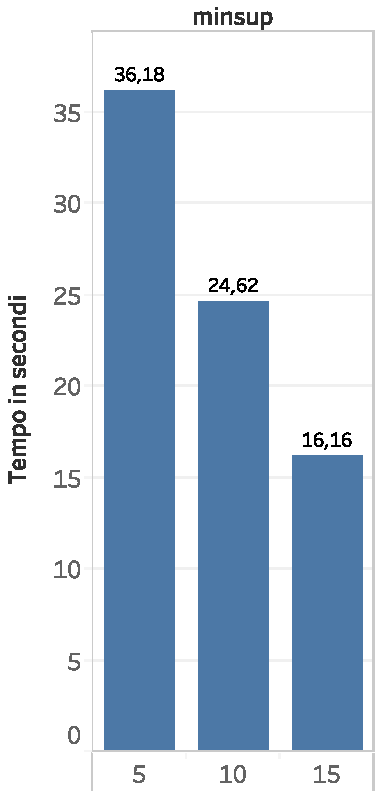
\includegraphics[scale=0.5]{res/fig/sec-4/performance/TimeMisupp.pdf}
   \caption{\(minsup\) tra \(5,10,15\)}%
  \label{fig:chap-4:TimeMinsupp}
  \end{subfigure}%
  \caption{Tempo di computazione alla variazione di \(minsize\) a sinistra e \(minsupp\) a destra}%
  \label{fig:chap-4:TimeMinsizeandMinsupp}
\end{figure}

Trattando poi dei parametri di continuità che riducono lo spazio di ricerca, \(\epsilon\) (\cref{fig:chap-4:TimeEpsilon}) presenta per entrambi i dataset una certa regolarità: al crescere del suo valore, aumenta il tempo di computazione.
Questa regolarità dipende dalla riduzione dello spazio di ricerca effettuato dai vincoli.
Valori più rigidi comportano una maggior riduzione dello spazio di ricerca, che si traduce in un pruning più forte

Su \(\tau\) (\cref{fig:chap-4:TimeTau}) la situazione è più eterogenea: non è possibile individuare un trend definito.
Ancora una volta le cause sono da ricercare nel debole pruning di \(\tau\), la presenza di questo vincolo infatti può in ceri casi rallentare l'esecuzione, in quanto giunge a risultati assimilabili a quelli ottenuti rilassando il vincolo.
Questa ricerca avviene in maniera più lenta, per via delle operazioni aggiuntive sul controllo della continuità.

\begin{figure}
  \centering
   \begin{subfigure}{.5\textwidth}
  \centering
    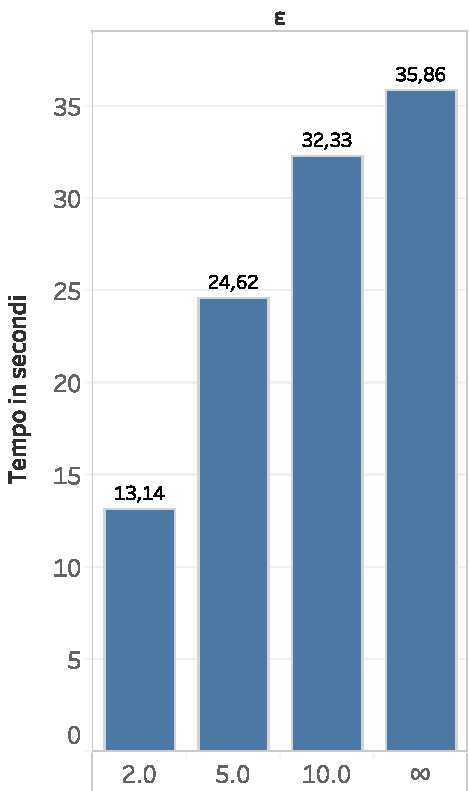
\includegraphics[scale=0.5]{res/fig/sec-4/performance/TimeEpsilon.pdf}
   \caption{\(\epsilon\) tra \(2,5,10,\infty\)}
  \label{fig:chap-4:TimeEpsilon}
\end{subfigure}%
\begin{subfigure}{.5\textwidth}
  \centering
   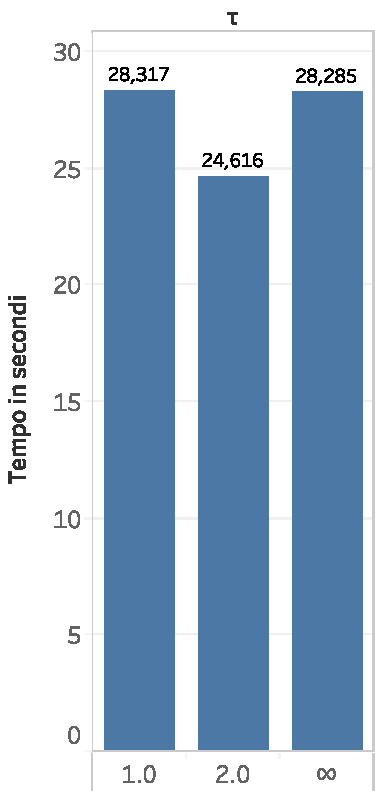
\includegraphics[scale=0.5]{res/fig/sec-4/performance/TimeTau.pdf}
   \caption{\(\tau\) tra \(1,2,\infty\)}%
  \label{fig:chap-4:TimeTau}
  \end{subfigure}%
  \caption{Tempo di computazione alla variazione di \(\epsilon\) a sinistra e \(\tau\) a destra}%
  \label{fig:chap-4:TimeEpsilonAndTau}
\end{figure}

Passando ai test di scalabilità, questi sono stati condotti su un sottoinsieme dei parametri utilizzati nella sezione precedente.
Ciascuna configurazione di parametri è stata testata variando rispettivamente il numero di executor  e quello di core, mantenendo come altri parametri i valori di default specificati nella \cref{tab:parameters-variation}.
La \cref{tab:cores-executors-variation} contiene i valori possibili per core e executor.

\begin{table}[H]
    \centering
   \begin{tabular}{||c c||}
 \hline
     Parametro & Valori \\ [0.4ex] 
 \hline\hline
   core & 2,\textbf{3},4 \\
 \hline
  executor & 5,\textbf{7},9 \\
 \hline
\end{tabular}
    \caption{Valori per core e executor (default in grassetto)}
    \label{tab:cores-executors-variation}
\end{table}


Le \cref{fig:chap-4:ScalabilityCORES,fig:chap-4:ScalabilityEXECUTORS}
mostrano i tempi di esecuzione alla variazione di questi parametri.

\begin{figure}
  \centering
   \begin{subfigure}{.5\textwidth}
  \centering
      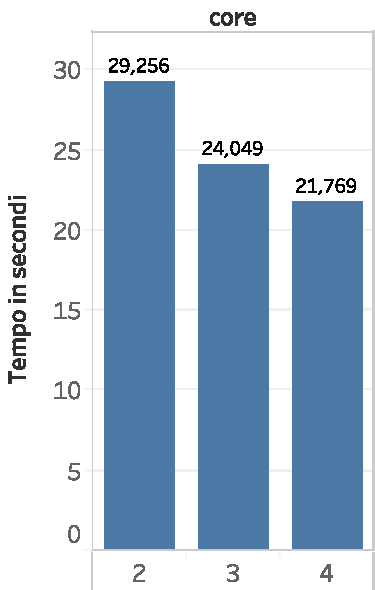
\includegraphics[scale=0.5]{res/fig/sec-4/scalability/ScalabilityDataCORES.pdf}
  \caption{core tra \(2,3,4\)}%
  \label{fig:chap-4:ScalabilityCORES}
\end{subfigure}%
\begin{subfigure}{.5\textwidth}
  \centering
   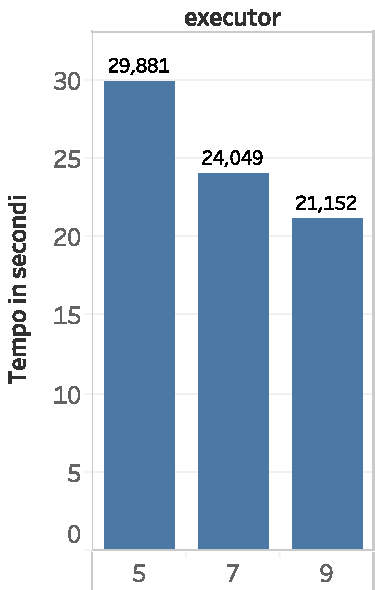
\includegraphics[scale=0.5]{res/fig/sec-4/scalability/ScalabilityDataEXECUTORS.pdf}
  \caption{executor tra \(5,7,9\)}%
  \label{fig:chap-4:ScalabilityEXECUTORS}
  \end{subfigure}%
  \caption{Tempo di computazione alla variazione di core a sinistra e executor a destra}%
  \label{fig:chap-4:ScalabilityCORESandEXECUTORS}
\end{figure}

Com'è possibile notare, la tendenza generale espressa dai grafici è una diminuzione dei tempi di esecuzione all'aumentare dell'impiego di risorse.

Infine per quanto riguarda l'ambito delle performance, sono stati eseguiti alcuni test di scalabilità rispetto al numero di traiettorie.
In particolare per questi è stato utilizzato Oldenburg, in quanto avente un numero di traiettorie molto superiore a Geolife.
La \cref{tab:variation-oldenburg} contiene i parametri di CUTE utilizzati durante queste esecuzioni.

\begin{table}[H]
    \centering
   \begin{tabular}{||c c||}
 \hline
     Parametro & Valore \\ [0.4ex] 
 \hline\hline
 traiettorie & \(50\)K,\(500\)K,\(1.000\)K \\
 \hline
 \(s\) & 1000 \\
 \hline
 \(t\) & 10 \\
 \hline
 \(minsize\) & 100 \\
 \hline
  \(minsupp\) & 10 \\
 \hline
  \(\epsilon\) & \(2\) \\
 \hline
 \(\tau\) & \(1\) \\
 \hline
   core & 3 \\
 \hline
  executor & 9 \\
 \hline
\end{tabular}
    \caption{Valori dei parametri di CUTE utilizzati durante i test sul numero di traiettorie su Oldenburg}
    \label{tab:variation-oldenburg}
\end{table}

I risultati indicano come a parità di risorse, CUTE riesca a gestire in tempi ragionevoli anche un numero di transazioni molto elevato (\cref{fig:chap-4:ScalabilityOldenburg}).
Nel caso peggiore infatti sono necessarie appena 10 minuti per eseguire la ricerca su un milione di traiettorie.
Questo dipende da diversi fattori.
In primo luogo il numero di celle, e di conseguenza quello di transazioni, rimane invariato durante le varie esecuzioni.
Ciò che cambia è quindi la lunghezza media di ogni transazione, che aumenta all'aumentare del numero di traiettorie.
Insiemi di transazioni di diversi ordini di grandezza vengono processati in diversi ordini temporali di grandezza.
Oltre a ciò, questi risultati possono essere collegati a valori molto stringenti per i parametri collegati al pruning, dimostrando così la loro efficacia nel ridurre lo spazio di ricerca.



\begin{figure}
  \centering
  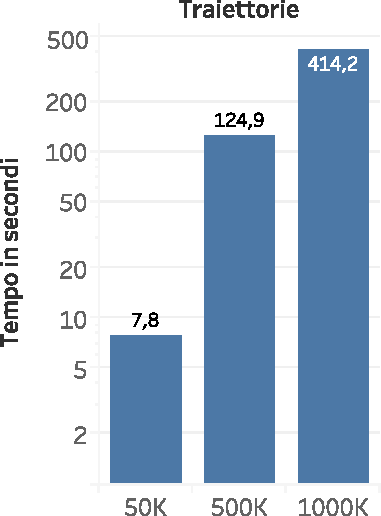
\includegraphics[scale=.5]{res/fig/sec-4/performance/ScalabilityOnOldenburg.pdf}
  \caption{Tempi di esecuzione in secondi variando il numero di traiettorie tra \(50\)K,\(500\)K,\(1000\)K}%
  \label{fig:chap-4:ScalabilityOldenburg}
\end{figure}

